
\subsection{Разработка структуры серверной части конструктора}


В данном разделе описываются разработанные структуры серверной части
конструктора и его основные алгоритмы функционирования.

\subsubsection{Модульная структура серверной части конструктора}

Модуль – набор структур и методов, который обобщает какую-то логику
приложения.

Модульная структура серверной части конструктора представлена на
рисунке~\ref{f:mod-server-struct}.

\begin{figure}[ht]
	\centering
	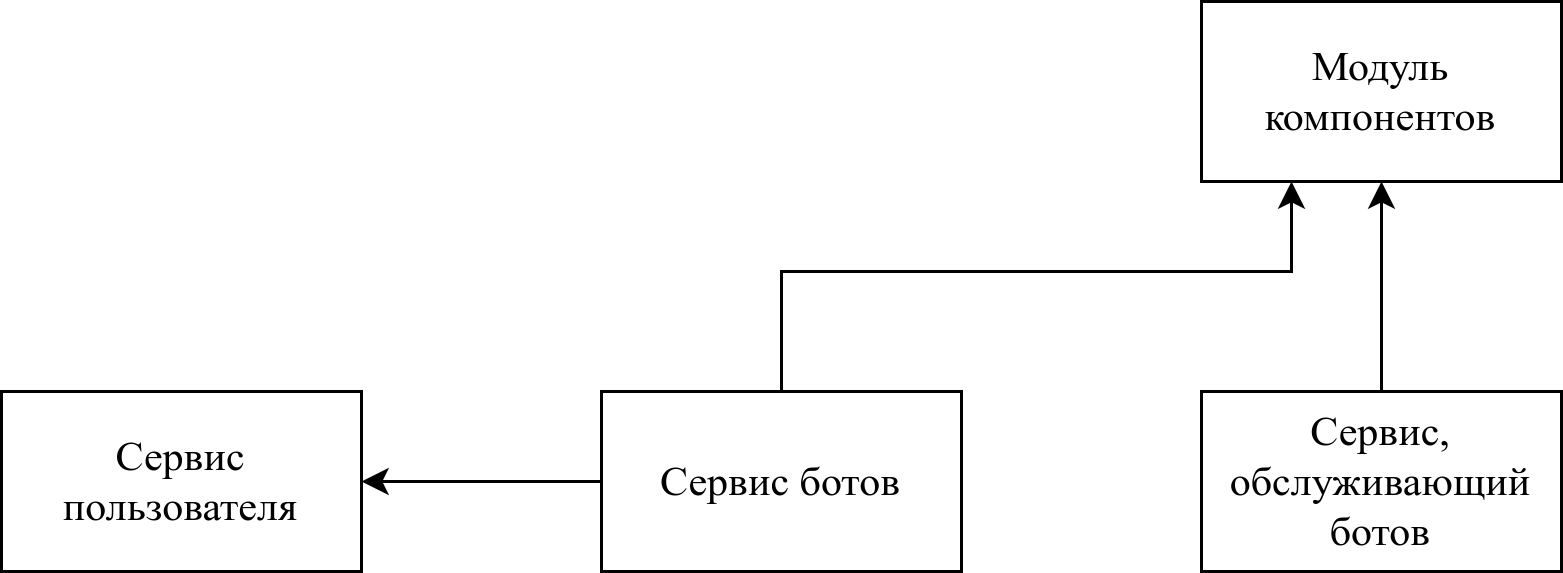
\includegraphics[width=0.8\textwidth]{mod-server-struct}
	\caption{Модульная структура серверной части конструктора}
	\label{f:mod-server-struct}
\end{figure}

Сервис ботов зависит от сервиса пользователей, который предоставляет
первому методы для авторизации пользователя. Также сервис ботов зависит
от модуля компонентов, который описывает структуры компонентов и
реализует их логику выполнения.

Для выполнения логики ботов сервис, обслуживающий ботов, вызывает
методы из модуля компонентов.

\subsubsection{Структура модуля компонентов}

Модуль компонентов состоит из следующих подмодулей:
\begin{itemize}
	\item подмодуль компонентов;
	\item подмодуль контекста;
	\item подмодуль исполнителя;
	\item подмодуль ввода-вывода.
\end{itemize}

Структура модуля компонентов представлена на рисунке~\ref{f:mod-comp-struct}.

\begin{figure}[ht]
	\centering
	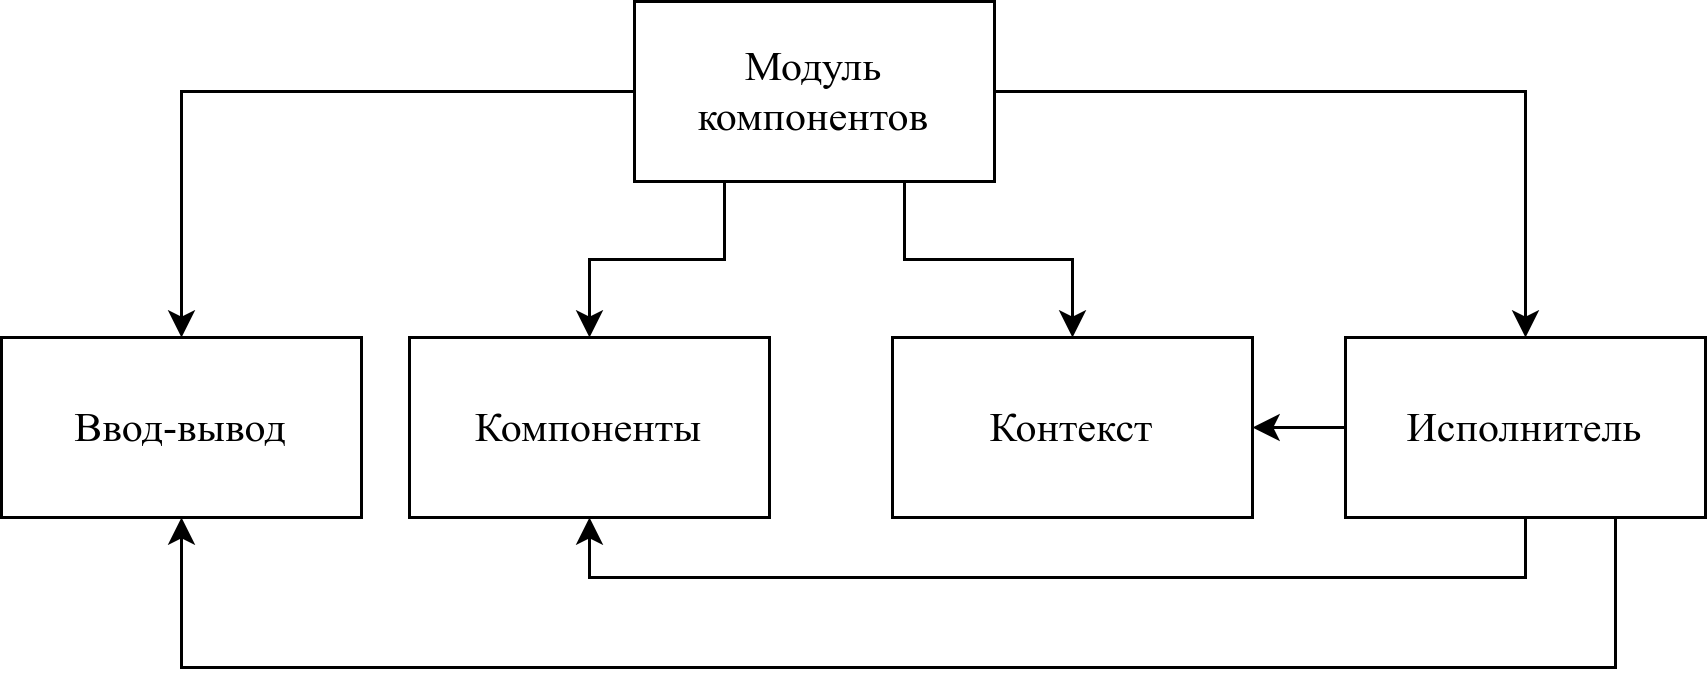
\includegraphics[width=0.8\textwidth]{mod-comp-struct}
	\caption{Структура модуля компонентов}
	\label{f:mod-comp-struct}
\end{figure}

Подмодуль компонентов содержит структуру и реализацию логики
компонентов. Каждый компонент реализует общий интерфейс компонента,
который определен в данном подмодуле.

В данном подмодуле определены следующие компоненты:
\begin{itemize}
	\item 	компонент ввода текста;
	\item 	компонент отправки сообщения;
	\item 	компонент вывода кнопок;
	\item 	компонент форматирования;
	\item 	компонент точки входа;
	\item 	компонент условия.
\end{itemize}

Подмодуль ввода-вывода предоставляет интерфейс, через который
окружение обменивается данными с рядом компонентов.

Подмодуль контекста содержит методы для работы с контекстом.
Контекст в рамках бота – память, с которой работают компоненты:
компоненты получают из контекста данные для выполнения и записывают в
него результат.

Исполнитель представляет собой объект, который содержит в себе
контекст и интерфейс ввода-вывода. Через него происходит выполнение
компонентов.


\subsubsection{Алгоритмы функционирования серверной части конструктора}

При взаимодействии Telegram пользователя с ботом происходит
отправка события сервису, обслуживающему ботов, который в дальнейшем
обрабатывает данное событие. Схема алгоритма обработки событий от
пользователя бота представлен на рисунке .
